% !TEX root = ../skript.tex

\chapter{GPS und Allgemeine Relativitätstheorie\label{chapter:thema}}
\lhead{GPS und Allgemeine Relativitätstheorie}
\begin{refsection}
\chapterauthor{Kevin Schmidiger}

\section{Einleitung}
Einsteins Allgemeine Relativitätstheorie war einer der Meilensteine der modernen Physik. Die Vereinigung von Raum und Zeit führte zu einem Neudenken in der Physik. Allerdings brachte es einige Konsequenzen mit sich, die in diesem Buch schon vorgestellt wurden. Dazu gehören die Längenkontaktion, die Verzerrung des Raumes für ein Objekt mit hoher Geschwindigkeit. Die Relativistische Masse; wenn man auf sein Gewicht achtet meidet man hohe Geschwindigkeiten. Und zu guter letzt, die Zeitdilatation, der Fluss der Zeit, beeinflusst durch die Geschwindigkeit und Gravitationsfeld. Auch in diesem Kapitel dreht es sich wieder um die Zeitdilatation.

Man stellt sich ja oft die Frage, Einsteins Theorie schön und gut, aber treffe ich den solche Effekte in meinem Alltag an? Die Antwort ist ja. Wie in dem Titel schon schliessen lässt, das GPS muss die Konsequenzen der Allgemeinen Relativität korrigieren, um die Position korrekt anzuzeigen. In diesem Kapitel wird genauer erläutert, wie das GPS die Allgemeine Relativität einbezieht und was das für Konsequenzen hätte, wenn Einstein nicht gewesen wäre.

\section{Das GPS (Global Positioning System)}
\rhead{GPS}
Als erstes muss man verstehen, wie das GPS eine Position bestimmt, damit man versteht warum die Allgemeine Relativitätstheorie hier greift. Das GPS besteht aus 24 Satelliten, welche die Erde so umkreisen, dass immer mindestens 4 Satelliten in Reichweite sind. Sprich, wo immer ich mich befinde, es sollten mindestens 4 Satelliten Verbindung zu mir haben. Damit bei Ausfällen keine Probleme auftreten, sind weitere 7 Satelliten im umlauf, die einsprigen könnten. Die Satelliten kreisen auf etwa 20'180 km Höhe. Dabei umkreisen sie die Erde 2 mal pro Tag. Grundsätzlich hat das GPS eine Genauigkeit von 10m. 

Was macht nun ein solcher Satellit? Der GPS Satellit hat unter anderem eine Atomuhr bei sich. Des weiteren weiss der Satellit immer was seine Positionsdaten sind. Die aktuellen Positionsdaten und seine aktuelle Zeit sendet er dann immer wieder richtung Erde. Dort kann dann ein GPS-Empfänger dann die Daten auswerten und seine Position bestimmen.

\subsection{Positionsbestimmung}
Wie wird nun die Position genau bestimmt? Wir suchen im Prinzip unsere Koordinaten unserer Position P(x,y,z). Im Prinzip sind die Position des GPS-Empfängers und die Position des Satelliten zwei Punkte und deren Distanz ist gleich

\begin{equation}
\label{eq:positioning}
    (x_i-x)^2 + (y_i-y)^2 + (z_i-z)^2 = c^2 (t_i -t).
\end{equation}

\noindent{}Wobei die indizierten Koordinaten die des Satelliten sind. Die Distanz lässt sich ermitteln durch die Zeit, die das Licht bzw. das Signal braucht, um beim Empfänger anzukommen. 
Anhand dieser Gleichung, sehen wir auch wieso es mindestens 4 Satelliten braucht, um die Position zu bestimmen. Einerseits brauchen wir die Koordinten x,y,z sowie die Zeit. Aber warum brauchen wir die Zeit des GPS-Empfängers? Wir messen die Distanz anhand der Zeit und der Lichtgeschwidigkeit. Und um dabei auf ein möglichst genaues Ergebnis zu kommen brauchen wir eine genaue Zeit. Der Empfänger hat natürlich keine Atomuhr (die würde definitiv zu viel Platz brauchen, sowie auch viel kosten). Also nutzen wir einfach die Mathematik, um die Zeit herauszufinden mit einer weiteren Gleichung. Es lässt sich also aus 4 Satelliten nun unsere gesuchte Position P(x,y,z) finden. 

\subsection{Distanz in Lichtsekunden}
Um das Ganze ein bisschen genauer zu verdeutlichen warum es wichtig ist, warum die Zeit möglichst genau sein muss, gehen wir ein bisschen genauer auf die linke Seite der Glechung \ref{eq:positioning} ein. Wir schauen mal wie weit das Licht in einer bestimmten Zeit kommt. Wir sollten nicht vergessen, das GPS hat eine Genauigkeit von 10m. Die Geschwindikeit des Lichtes beträgt  \(c = 2.9979 * 10^8 m/s\). \\

\begin{center}
\begin{tabular}{| c | c |}
\hline
Zeit & Distanz \\
\hline
1s & 7.5 Erdumrundungen / fast Erde - Mond \\
\hline
1ms & 300km \\
\hline
1$\mu$s & 300m \\
\hline
1ns & 0.3m \\
\hline
\end{tabular}
\end{center}

\noindent{}Wir sehen hier, wenn wir eine Abweichung von nur einer Nanosekunde(!) haben, dann ensteht eine Ungenauigkeit von 0.3m. Das sind 0.000'000'001s. Für das GPS würde das bedeuten, dass die Zeit maximal 33ns Abweichen darf.

\section{Zeitdilatation beim GPS}
Beim GPS haben wir zwei Faktoren, die die Zeit des GPS Satelliten beeinflussen. Zum einen durch die Geschwindigkeit und zum einen die durch das Gravitationsfeld der Erde. Beide greifen sich gegenseitig an. Wir schauen zuerst jede Zeitdilatation einzeln an und schauen was für eine Gesamtdilatation herauskommt. Wir beginnen mit der einfacheren, der durch die Geschwindigkeit und dann schauen wir die des Gravitationsfeldes an.

\subsection{Zeitdilatation duch Geschwindigkeit}
\rhead{Zeitdilatation duch Geschwindigkeit}
Wir erinnern uns an den Relativitätsfaktor

\begin{equation}
\label{eq:realativityfac}
\gamma = \frac{1}{\sqrt{1 - \frac{v^2}{c^2}}}.
\end{equation}

\noindent{}Wie schon füher besprochen ist der Faktor grösser wenn die Geschwindigkeit sich der Lichteschwindigkeit nähert. Setzten wir für die Gleichung \ref{eq:realativityfac} folgende Grössen ein. Der Satellit kreist mit einer Geschwindigkeit von \(v \approx 3874 m/s \). Das ist eine ziemlich kleine Geschwindigkeit verglichen mit der Lichtgeschwindigeit, aber schauen wir mal was das Ergebnis sagt. Und die Lichgeschwindigkeit wie gehabt \(c = 2.9979 * 10^8 m/s\). 
Rechnen wir das nun aus ergibt es folgendes:\\

\(\gamma = \frac{1}{\sqrt{1 - \frac{v^2}{c^2}}} = \frac{1}{\sqrt{1 - \frac{3874 \frac{m}{s}^2}{(2.9979 * 10^8 \frac{m}{s} )^2}}} = 1 + 83.4939 * 10^{-12} \) \\

\noindent{}Das heisst nun für eine Sekunde hier auf der Erde geht die Zeit für den Satellit Aufgrund der Geschwindigkeit die Zeit um \( \frac{1}{\gamma}\) langsamer. Ausgerechnet sind das für eine Sekunde: \\

\( \Delta t = \frac{1}{\gamma} * t_0 = \frac{1}{1 + 83.4939 * 10^{-12}} * 1s = 1 - 83.4939 * 10^{-12}s \) \\

\noindent{}Momentan wäre das eine Abweichung von 2.5cm pro Sekunde. Rechnen wir beides, die Zeitdilatation und die Distanzzabweichung auf einen Tag aus erhalten wir:\\

\( t_{tot} = \Delta t * 60 * 60 * 24 = 7.2138  \frac{\mu s}{d} \) bzw. \\

\( l_{tot} = \Delta l * 60 * 60 * 24 = 2.164 \frac{km}{d} \) \\

\noindent{}Nach etwas mehr als 6min sind die 10m Genauigkeit nur Aufgrund der Geschwindigkeit dahin. Auf längere Zeit gesehen wäre dann das GPS unbrauchbar. Soweit zur Zeitdilatation durch die Geschwindikeit.

\subsection{Zeitdilatation duch Gravitation}
\rhead{Zeitdilatation duch Gravitation}
Dieser Teil ist wesentlich komplizierter zu verstehen. Als erstes müssen wir uns im klaren sein, was wir eigentlich wissen wollen. Und zwar die Zeitdilatation des Satelliten aufgrund der Graviatition der Erde. Wir erinnern uns an die Schwarzschild-Metrik, welche eine Lösung für die Einsteinschen Feldgleichungen ist, die sich mit der Zeit nicht ändert. Die Metrik wurde schon als Gleichung in \ref{skript:schwarzschild:kugelsymmetrischeloesung} gezeigt, ist hier aber zur Übersicht nochmal als Matrix dargestellt. \\

\begin{equation}
\frac{\partial g_{\mu\nu}}{\partial t}= 
\begin{pmatrix}
-\biggl(1-\frac{r_g}r\biggr)c^2 & 0 & 0 & 0 \\
0 & \frac1{\displaystyle 1-\frac{r_g}r} & 0 & 0 \\
0 & 0 &  r^2 & 0 \\
0 & 0 & 0 & r^2 (d\vartheta^2 + \sin^2\vartheta) \\
\end{pmatrix}
= 0
\end{equation} \\

\noindent{}Wie schon in Kaptiel \ref{skript:chapter:schwarzschild} erwähnt, ist dies eine kugelsymmetrische Lösung. Diese kann als Approximation in der Umgebung von Massereichen Objekten benutzt werden, wobei die Eigenrotation, der Objekte nicht miteinbezogen ist. In der Metrik sieht man, dass Kugelkoordinaten eine Rolle spielen und deswegen noch eine veranschaulichung wie Kugelkoordinaten sich zusammensetzen.

\begin{figure}[h]
    \centering
    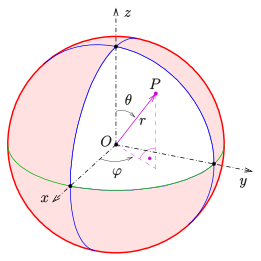
\includegraphics[width=0.5\textwidth]{gps/pictures/kugelkoordinaten.png}
    \caption{Kugelkoordinaten}
%Bild:https://de.wikipedia.org/wiki/Kugelkoordinaten
\end{figure}

In unserem Falle zusammen mit der Schwarzschild-Metrik ist \( r \) der Radius vom Erdmittelpunkt zum Satelliten. \( \Theta \) (in der Metrik \( \vartheta \)) entspricht quasi den Breitengraden, nur dass es von oben nach unten geht bzw von 0 bis \( \pi \). \( \varphi \) entspicht quasi den Längengraden und geht von 0 bis 2\( \pi \). Mit den Kogelkoordinaten können wir die Kreisbahn des Satelliten als Geodäte beschreiben. Rechnet man die Christoffelsymbole für die Schwarzschild-Metrik mithilfe von Maxima o. Ä. aus und setzt diese in die Geodätengleichung ein erhält man folgende Gleichungen:

\begin{align*}
\ddot t(s)
&=
-\frac{1}{1-\displaystyle\frac{r_g}{r}}\frac{r_g}{r}\frac{1}{r}\dot t(s)\,\dot r(s)
\\
\ddot r(s)
&=
-\biggl(1-\frac{r_g}{r}\biggr)\frac{r_g}{r}\frac1{2r}\dot t(s)^2
+\frac{1}{1-\displaystyle\frac{r_g}{r}} \frac{r_g}{r}\frac1{2r}\dot r(s)^2
-(r_g-r)\dot \vartheta(s)^2 + (r_g-r)\sin^2 \vartheta \cdot \dot \varphi(s)^2
\\
\ddot \vartheta(s)
&=
-\frac{2}{r} \dot r(s)\, \dot \vartheta(s)
+\cos\vartheta\sin\vartheta \cdot \dot\varphi(s)^2
\\
\ddot \varphi(s)
&=
-\frac{2}{r} \dot r(s)\,\dot \varphi(s)
-2\cot\vartheta \cdot \dot r(s)\,\dot\varphi(s)
\end{align*}

\noindent{}Diese Gleichungen wurden schon im Kapitel \ref{skript:schwarzschild:geodaetengleichung} hergeleitet. 

Schauen wir, was wir nun mit den Gleichungen anfangen können. Nehmen wir einen Satelliten, der um den Äquator kreist. Es gilt also folgendes: \\

\begin{align*}
t &= ges. &
r &= r_{Erde} + h_{Satellit} = const \\
\theta &= \frac{\pi}{2} = const &
\phi &= 0..2\pi = unbek.
\end{align*}

\noindent{}Wir sind auf der Suche nach der Zeitdilatation also wissen wir nicht was \( t \) ist. Wir wissen aber \(  r \) und \( \vartheta \). Bei \( \varphi \) hingegen wissen wir nicht genau wo der Satellit sich befindet zur Zeit t befindet. Wir lassen \( \varphi \) daher mal als unbekannt stehen. Berücksichtigen wir all dies in den Geodätengleichungen fallen alle Terme mit \( \dot r(s) \) und \( \dot \vartheta (s) \) weg, denn deren Ableitungen sind 0. Des weiteren fallen die Terme mit \( \cos \vartheta \) weg, denn \( \cos \frac{\pi}{2} = 0 \). Die Geodätengleichungen sehen nun wie folgt aus:

\begin{align*}
\ddot t(s) &= 0 \\
\ddot r(s)
&=
-\biggl(1-\frac{r_g}{r}\biggr)\frac{r_g}{r}\frac1{2r}\dot t(s)^2
+ (r_g-r)\sin^2 \vartheta \cdot \dot \varphi(s)^2 \\
\ddot \vartheta(s) &= 0 \\
\ddot \varphi(s) &= 0
\end{align*}

\noindent{}Die einzig aussagekräftige Gleichung die Übrig bleibt ist \( \ddot r(s) \). In der Gelcihung haben wir sogar eine Beziehung \( \dot t \) und \( \dot \varphi \). Wenn wir die Gleichung noch ewas weiter bearbeiten, dann sieht diese wie folgt aus:

\begin{equation}
0 = -\biggl(1-\frac{r_g}{r}\biggr)\frac{r_g}{r}\frac1{2r}\dot t(s)^2 + (r_g-r)\cdot \dot \varphi(s)^2
\end{equation}

\noindent{}Da \( \dot r(s) = 0 \) ist somit \(  \ddot r(s) = 0 \). Zudem ist \( \sin \vartheta = \sin \frac{\pi}{2} = 1 \) und kann daher vereinfacht werden. Nun haben wir eine Gleichung aber noch zwei Unbekannte. Um diese zu lösen brauchen wir noch eine zweite. Erinnern wir uns daran, dass die Lichtgeschwindigkeit absolut ist. Möchte nun man nun von einem Vektor seine Länge messen gilt folgende Gleichung, welche in Kapitel \ref{skript:speziell:energieimpuls} schon gezeigt wurde:

\begin{equation}
g_{\mu\nu}u^\mu u^\nu=-c^2 \\
\end{equation}

\noindent{}Das ist eine vom Koordinatensytemunabhängige Grösse. Möchte man eine Längenmessung machen erhält man folgende Gleichung: \\

\begin{equation}
ds^2 = g_{\mu\nu}du^\mu du^\nu = -c^2
\end{equation}

In unserem Fall gilt \( g_{\mu\nu} \) entspricht der Schwarzschild-Metrik und \( u \) entspricht der Position des Satelliten. \\

\begin{align*}
g_{\mu\nu} &= 
\begin{pmatrix}
-\biggl(1-\frac{r_g}r\biggr)c^2 & 0 & 0 & 0 \\
0 & \frac1{\displaystyle 1-\frac{r_g}r} & 0 & 0 \\
0 & 0 &  r^2 & 0 \\
0 & 0 & 0 &  r^2(d\vartheta^2 + \sin^2\vartheta) \\
\end{pmatrix} &
u &= 
\begin{pmatrix}
t(s) \\
r(s) \\
\vartheta (s) \\
\varphi (s)
\end{pmatrix} = 
\begin{pmatrix}
\dot t(s) \\
\dot r(s) \\
\dot \vartheta (s) \\
\dot \varphi (s)
\end{pmatrix}
\end{align*}

\noindent{}Da wir wegen der Geodätengleichung jeweils die Komponenten des Positionsvektors abgeleitet haben nutzen wir diese. Setzen wir alles ein ergibt sich folgende Gleichung: \\

\( -\biggl(1-\frac{r_g}r\biggr)c^2 \dot t(s)^2 +  \frac1{\displaystyle 1-\frac{r_g}r} \dot r(s)^2 + r^2 \dot \vartheta(s)^2 + r^2 \dot \vartheta + r^2 \sin^2 \vartheta \dot \varphi (s)^2 = -c^2 \) \\

\noindent{}Vereinfachen wir die Gleichung noch, denn \( \dot r(s) = 0 \), \( \dot \vartheta(s) = 0 \) und \( \sin \vartheta = \sin \frac{\pi}{2} = 1 \) dann erhalten wir:

\begin{equation}
-\biggl(1-\frac{r_g}r\biggr)c^2 \dot t(s)^2 + r^2  \dot \varphi (s)^2 = -c^2 
\end{equation}

\noindent{}Und auch hier haben wir wieder eine Beziehung zwischen \( \dot t(s) \) und \( \dot \varphi(s) \). Jetzt haben wir zwei Gleichungen mit zwei Unbekannten. Da wir \( \dot t(s) \) suchen, setzen wir \( \dot \varphi(s) \) ein und lösen nach \( \dot t(s) \) auf. Nachdem alles Umgestellt und vereinfacht wurde erhalten wir folgende Gleichung:

\begin{equation}
\label{gps:equation:gravidilatation}
\dot t(s) = \tau = \frac{1}{\sqrt{1-\frac{r_g}{r}}}
\end{equation}

\noindent{}Intressanterweise sieht das sehr ähnlich dem Relativitätsfaktor aus \ref{eq:realativityfac} aus. Nur das hier nicht die Geschwindigkeit eine Rolle spielt sondern der Abstand zu einem Massereichen Objekt. Je grösser die Entfernung zum Objekt desto weniger hat das Gravitationsfeld Einfluss auf die Zeit. 

So, jetzt haben wir eine schöne einfache Gleichung und dann können wir nun ausrechnen was für eine Zeitdilatation ensteht durch das Gravitationsfeld. Der Schwarzschildradius welcher schon in Kaptiel \ref{skript:schwarzschild:rg} kennengelernt. Dieser ist bektanntlich:

\begin{equation}
 r_g=\frac{2MG}{c^2}
\end{equation}

\noindent{}Dabei ist \( M = m_Erde = 5.972 * 10^{24}kg \), \( G = 6.673 \frac{Nm^2}{kg^2} = \) Gravitationskonstante und wie gehabt \( c = 2.9970 * 10^8 \frac{m}{s} \). Setzten wir das in die Gleichung ein ergibt das folgendes:\\

\( r_g=\frac{2MG}{c^2} = \frac{2 * 5.972 * 10^{24}kg *  6.673 \frac{Nm^2}{kg^2}}{ (2.9970 * 10^8 \frac{m}{s})^2} = 8.868 * 10^{-3}m = 8.87mm\) \\

Die Gleichung \ref{gps:equation:gravidilatation} bezieht sich ja immer auf die Distanz zu einem Masseereichem Objekt. Genaugenommen zu dem Gravitationszentrum des Massereichen Objektes. Das heisst, im Prinzip haben wir auf der Erdoberfläche auch schon eine Zeitdilatation gegenüber dem Erdmittelpunkt. Da sich unsere Position ja grundsätzlich auf der Erdoberfläche befindet müssen wir das auch noch berücksichtigen. Um also die gesamte Zeitdilatation in Berücksichtigung auf die Erdoberfläche zu erhalten müssen wir die Zeiltdilatation auf der Erdoberfläche von der Zeitdilatation von dem Satelliten abziehen. Das sieht wie folgt aus: \\

\( \dot t(s)_ {ges} = \tau = \frac{1}{\sqrt{1-\frac{r_g}{r_{Erde}}}} - \frac{1}{\sqrt{1-\frac{r_g}{r_{Satellit}}}} \) \\

Die Satelliten Kreisen in einer Höhe von 20 200km über der Erdoberfläche. Der Radius ist allerdings auf das Gravitationszentrum bezogen, also müssen wir den Radius der Erde zum Mittelpunkt dazu addieren und dann erhalten wir den gesamt Radius von \( r_tot = r = h_{Satellit} + r_{Erde} = r = 20.200 km + 6,371 km = 20.2 * 10^6m + 6.371 * 10^3m = 26.571 * 10^6m \). Setzten wir nun diese erlangten Grössen ein erhalten wir:\\

\( \dot t(s)_ {ges} = \tau = \frac{1}{\sqrt{1-\frac{r_g}{r_{Erde}}}} - \frac{1}{\sqrt{1-\frac{r_g}{r_{Satellit}}}} =  
\frac{1}{\sqrt{1-\frac{8.868 * 10^{-3}m}{ 6.371 * 10^3m}}} - \frac{1}{\sqrt{1-\frac{8.868 * 10^{-3}m}{ 26.571 * 10^6m}}} =  529.09 * 10^{-12} \) \\

Im Prinzip bedeutet das nun, dass eine Sekunde auf der Erde \( 529.09ps \) länger dauert als auf dem Satellit. Den je näher man einem Massereichem Objekt ist, desto langsamer vergeht die Zeit, abhängig von seiner Masse. Das entspricht einer Abweichung von 15.9cm. pro Sekunde. Rechnet man dies auch wieder auf den ganzen Tag hoch erhält man: \\

\( t_{tot} = 529.09 * 10^{-12} * 60 * 60 * 24 = 45.713\frac{\mu{}s}{d} \) \\

\( l_{tot} = 0.3 * 10^{-3} * 60 * 60 * 24 = 13.714\frac{km}{d} \) \\

\section{Gesamte Zeitdilatation}
\rhead{Gesamte Zeitdilatation}
Die beiden Effekte greifen sich Gegenseitig an. Als erstes haben wir uns mit der Zeitdilatation durch Geschwindigkeit beschäftigt. Dabei ging es ja darum, dass der Satellit einen Zeitunterschied gegenüber jemandem der sich langsamer oder gar nicht fortbewegt. Wegen der höheren Geschwindigkeit des Satelliten gegenüber einem ruhendem Objekt, vergeht dessen Zeit langsamer. Gegenüber die Zeitdilatation durch die Gravitation, welche die Zeit langsamer vergehen lässt je näher man sich einem Massereichem Objekt aufhält. Wir auf der Erdoberfläche befinden uns näher am Gravitationszentrum als der Satellit. Das bedeutet gegenüber dem Satelliten verläuft unsere Zeit langsamer. Zusammengefasst heisst das, beim Satelliten läuft die Zeit schneller, da er weiter vom Gravitationszentrum ist, aber wegen seiner Geschwindikeit wird seine Zeit gebremst.

\begin{equation}
\tau_{tot} = \tau_{Gavitation} - \tau_{Geschwindikeit}\\
\end{equation}

\noindent{}Wenn man die Zahlen einsetzt erhält man:\\

\(  529.09 "10^{-12}  -  83.49 * 10^{-12}s =  445.6 * 10^{-12}s  \) \\

\(  45.713\mu{}s - 7.213\mu{}s = 38.5\frac{\mu{}s}{d} \) \\

\noindent{}Das entsricht einer Abweichung von 11.5km pro tag. bzw. 13.37cm pro Sekunde. 

Um diese Zeitdifferenz zu vermeiden, müssen die Satelliten ständig ihre Zeit anpassen. Hätte Einstein nicht diese Entdeckung gemacht hätte man vielleicht nicht verstanden, warum das GPS immer eine falsche Position anzeigt. 

\section{Zahlenspielereien}
Zurück zu der Frage, wo man im alltag auf die Effekte der Allgemeinen Relativitätstheorie stösst, das GPS ist ein Beispiel. Das Beispiel zeigt aber auch, dass wenn man nicht eine besonders hohe Geschwindigkeit hat oder sich in der Nähe eines besonders Massereichem Objekt befindet, die Effekte extrem klein sind. Sie sind so minimal, dass man sie eigentlich ausser Acht lassen kann. Beim GPS geht das halt nicht, da es tatsächlich nicht klarkommen würde, aber für einen Astronauten in der ISS spielt der Effekt keine Rolle. Selbst wenn dieser sich ein paar Wochen auf der Station befindet, und dann zur Erde zurück kehrt ist der Zeitunterschied immernoch sehr sehr klein. Wir können das ja mal ausprobieren.

\subsection{Zeitdilatation eines Astronauten der ISS}
\rhead{Zeitdilatation eines Astronauten der ISS}
Die ISS kreis auf einer durchschnittlichen Orbitalhöhe von \( h_{ISS} = 400km \). Die ISS ist viel näher als der GPS Satellit, das heisst der Effekt duch die Gravitation dürfte kleiner sein als dem des Satelliten. Ihre Geschwindikeit beträgt etwa \( v = 28'000\frac{km}{h} = 7777.77\frac{m}{s} \). Die Geschwindikeit hingegen ist viel höher als die des Satelliten, also dürfte hier der Effekt gösser sein. Nutzen wir diese Daten können wir die beiden Zeitdilatationen ausrechen.\\

\( \tau_{Geschwi} =  \frac{1}{\sqrt{1 - \frac{v^2}{c^2}}} = \frac{1}{\sqrt{1 - \frac{( 7777.77\frac{m}{s})^2}{c^2}}} = 3.025 * 10^{-9}s\) \\

\( \tau_{Gravi}= \tau = \frac{1}{\sqrt{1-\frac{r_g}{r_{Erde}}}} - \frac{1}{\sqrt{1-\frac{r_g}{r_{ISS}}}} 
= \frac{1}{\sqrt{1-\frac{r_g}{6371 * 10^3}}} - \frac{1}{\sqrt{1-\frac{r_g}{6371 * 10^3 + 400 * 10^3}}} = 41.115 * 10^{-12}s \) \\

\noindent{}Daraus resultiert eine Gesamt Zeitdilatation von:\\

\( \tau_{ges} = \tau_{Gravi} - \tau_{Geschwi} = -2.989 * 10^{-9} \) \\

\noindent{}Hoppla! Was ist denn das für ein Ergebnis. Naja, wenn man sich die Zahlen der beiden Dilatationen anschaut, dann wir einem klar, dass die Gravitation einen kleineren Einfluss hat als die, der Geschwindikeit. Also kann man hier sagen, dass dem Astronaut Zeit geschenkt wird. Seine Zeit läuft langsamer als die Zeit auf der Erdoberfläche. Rechnet man dies auf einen typisch halbjährigen Aufenthalt in der ISS aus erhält man:\\

\( -2.989 * 10^{-9} * 60 * 60 * 24 * 180 = -0.0464s \) \\

\noindent{}Das ist immer noch weit von einem spürbarem Effekt. Also selbst für einen Astronauten spielt die Zeitdilatation jetzt durch Geschwindigkeit keine Rolle.

\subsection{GPS mit Sonne als Gravitationsfeld}
\rhead{GPS mit Sonne als Gravitationsfeld}
Wir haben jetzt immer die Erde als Gravitationsfeld benutzt. Schauen wir mal was das für das GPS bedeuten würde, wenn unser Planet gleich der Sonne wäre. Die Masse der Sonne ist \( m_{Sonne} = 1.989 * 10^30kg \) der Radius ist \( r_{Sonne} = 6.96 * 10^8m \) und der Schwarzschildradius ist \( r_g = \frac{2GM}{c^2} = 2.954 * 10^3m \). Gehen wir davon aus dass der Satellit diesselbe Geschwindikeit hat und die Gleiche höhe. Setzen wir wiederum die Zahlen ein ergibt dies:\\

\( \tau_{Geschw} = \frac{1}{\sqrt{1 - \frac{v^2}{c^2}}} = \frac{1}{\sqrt{1 - \frac{3874 \frac{m}{s}^2}{(2.9979 * 10^8 \frac{m}{s} )^2}}} = 83.4939 * 10^{-12}s \) \\

\( \tau_{Gravi} = \frac{1}{\sqrt{1-\frac{r_g}{r_{Sonne}}}} - \frac{1}{\sqrt{1-\frac{r_g}{r_{Satellit}}}} =  
\frac{1}{\sqrt{1-\frac{2.954 * 10^3m}{6.96 * 10^8m}}} - \frac{1}{\sqrt{1-\frac{2.954 * 10^3m}{ 6.96 * 10^8m + 20.2 * 10^6}}} =  59.85 * 10^{-9}s \)\\

\noindent{}Das ergibt eine gesamt Zeitdilatation von \( \tau_{ges} = 59.85 * 10^{-9}s = 59.85ns \), da der Faktor der Geschwindigkeit fast nichts ausmacht. Das sind dann schon 18m pro Sekunde Abweichung nur wegen der Gravitation. 

Aber auch hier die Zeitliche Abweichung ist sehr gering und würde nicht allzuviel ausmachen, auch auf längere Sicht gesehen. Die Effekte sind zwar sehr klein bei nicht sehr Massereichen Objekten oder kleinen Geschwindigkeiten, sind jedoch Systeme von der Zeit abhängig dann stellt sich die Frage wie genau, bzw. ungenau es sein darf. Denn wenn wie beim GPS die Zeit eine sehr grosse Rolle spielt, dann kann es sein, dass man die Allgemeine Relativitätstheorie miteinbeziehen muss.

\printbibliography[heading=subbibliography]
\end{refsection}
